%!TEX root = paper.tex
%%%%%%%%%%%%%%%%%%%%%%%%%%%%%%%%%%%%%%%%%%%%%%%%%%%%%%%%%%%%%%%%%%%%%%%%%%%%%%%%
\section{Simulation and Scenario Evaluation}
\label{sec:simulation}

Based on the model introduced in Section~\ref{sec:model} a stochastic \gls{DES} was created that implements this model. This R-based simulator strifes to translate all of the earlier discussed lag blocks, while keeping them as configurable as possible.

By using a vector-based statistics language the core loop is kept compact and easy to modify and reorder to adapt to new scenarios in addition to the ones evaluated here. Due to the influence of several stochastic processes and the differing offset of the clocked processes, a sufficient number of repetitions is required to provide meaningful results. This is achieved by running large numbers of simulations in parallel through the built-in R facilities. Therefore, the evaluation of the presented scenarios was each conducted with $1000$ repetitions.

This section presents simulation results on each of the flavors of how to play video games: the local, online, and the cloud scenario.

The investigations here are not intended to cover every aspect of all parameters or to conduct full parameter studies, but are rather intended to highlight some particular aspect in each of the scenario. 

All of the source code and the data from the upcoming scenarios is provided in the simulation-folder\footnote{\url{https://github.com/mas-ude/onlinegame-lag-sim/tree/master/simulation}} of the repository and can be used as public domain.


\subsection{Parameters}

Besides being fully reconfigurable, the simulation currently also has a few default parameters set and makes assumptions that go beyond what the base end-to-end model implies for reasons of simplicity. They are briefly covered here.

First, the input is modeled by an exponential distribution with a rate of $20$ events per second. The offsets between the clocked processes are uniformly distributed in their respective intervals. It is further assumed, that the server processes each tick in a truncated normal distribution duration with $\mu = \SI{3}{\milli\second}$ and $\sigma = \SI{0.1}{\milli\second}$.
%\textbf{TODO:} implications and reasons?
Additionally, the rate at which command messages are sent to the game server is set equal to the server's tickrate as the server would not process more commands either way. This might however increase the end-to-end lag in some situations if a command message just misses one of the server's ticks and has to wait another full cycle.


%%%%%%%%%%%%%%%%%%%%%%%%%%%%%%%%%%%%%%%%%%%%%%%%%%%%%%%%%%%%%%%%%%%%%%%%%%%%%%%%
\subsection{Local Games}

The first and simplest scenario to be investigated here, is the case of the local game. In the version implemented here, the tickrate is still present, but the influence of the network is entirely removed. It therefore represents the best-case an online multiplayer game could achieve, when the server would run locally.

\begin{figure}[!t]
	\centering
	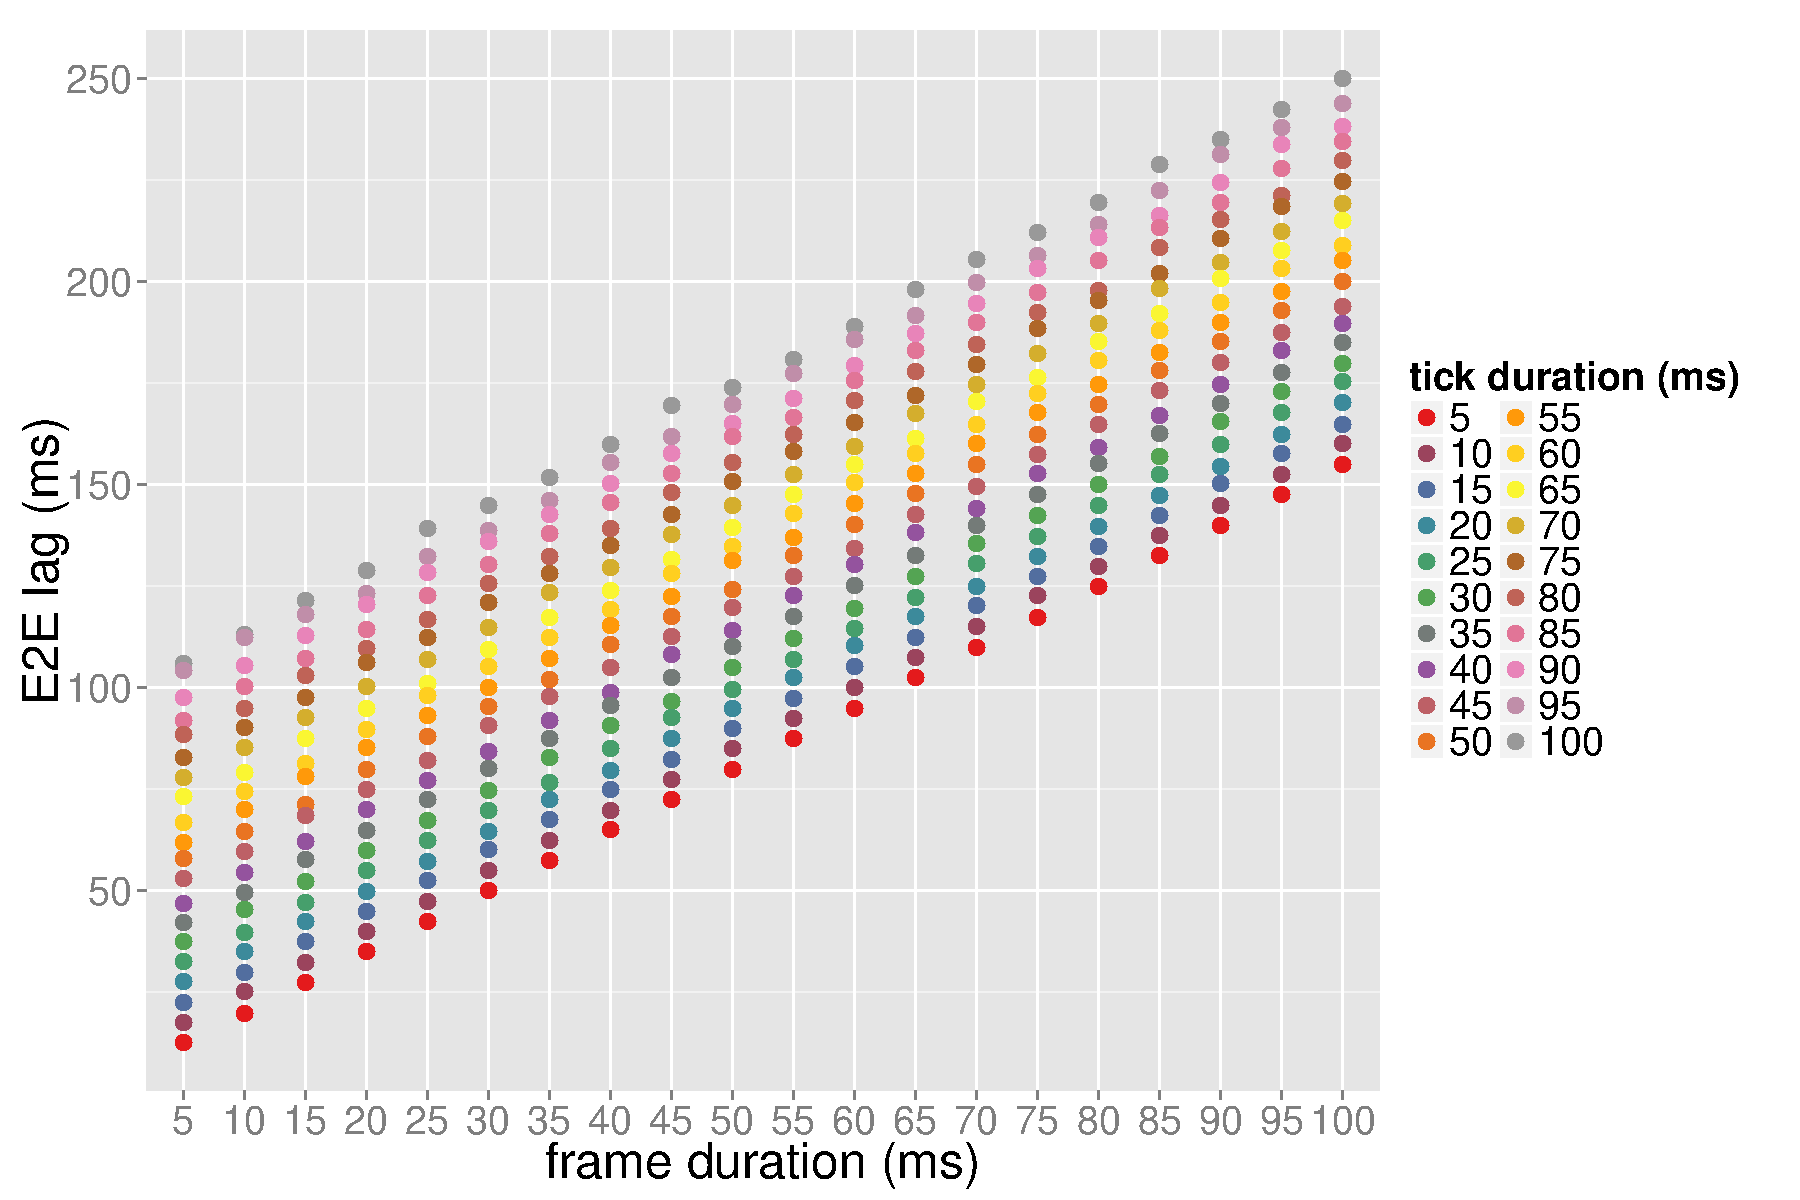
\includegraphics[width=1.0\columnwidth]{../simulation/visualization/nwless-onlinegame-1000rounds.pdf}
	\caption{Scatterplot of the median E2E lag under various frame and tick durations in a scenario where the game is running fully local.}
\label{fig:nwless-scatter}
\end{figure}

Figure~\ref{fig:nwless-scatter} presents a scatter plot of the relationship between the frame duration (i.e., the inverse of the framerate), the tick duration, and the resulting end-to-end lag. The offset between the command message, tickrate, and framerate is responsible for this lower limit of lag and results in lag values generally much higher than just the sum of the tick and frame duration.

Looking at a typical \SI{60}{\hertz} video game with an equal tickrate (i.e. a frame duration of $\approx \SI{16.6}{\milli\second}$) the results for the lag are in the range of \SIrange{45}{50}{\milli\second}. So even under quasi-optimal circumstances, there is already a considerable amount of end-to-end lag (especially considering that the simulation model does not factor in the delay of the screen and input devices) that can only get worse with the presence of network delay. Therefore, video games, and quality assessments thereof, should try to achieve the highest framerate possible to minimize this influence.

%%%%%%%%%%%%%%%%%%%%%%%%%%%%%%%%%%%%%%%%%%%%%%%%%%%%%%%%%%%%%%%%%%%%%%%%%%%%%%%%
\subsection{Online Gaming}

Next up is the full scenario of an online video game, now with the network lag included. For this exemplary scenario, the one-way delay was assumed to follow a truncated normal distribution with $\mu = \SI{20}{\milli\second}$ and $\sigma = \SI{5}{\milli\second}$, producing no negative results. Typical, competitive online games today are expected to operate in such ranges, while a \acrshort{RTT} of \SI{100}{\milli\second} is often considered to be the upper limit for a good playing experience for many games.

\begin{figure}[!t]
	\centering
	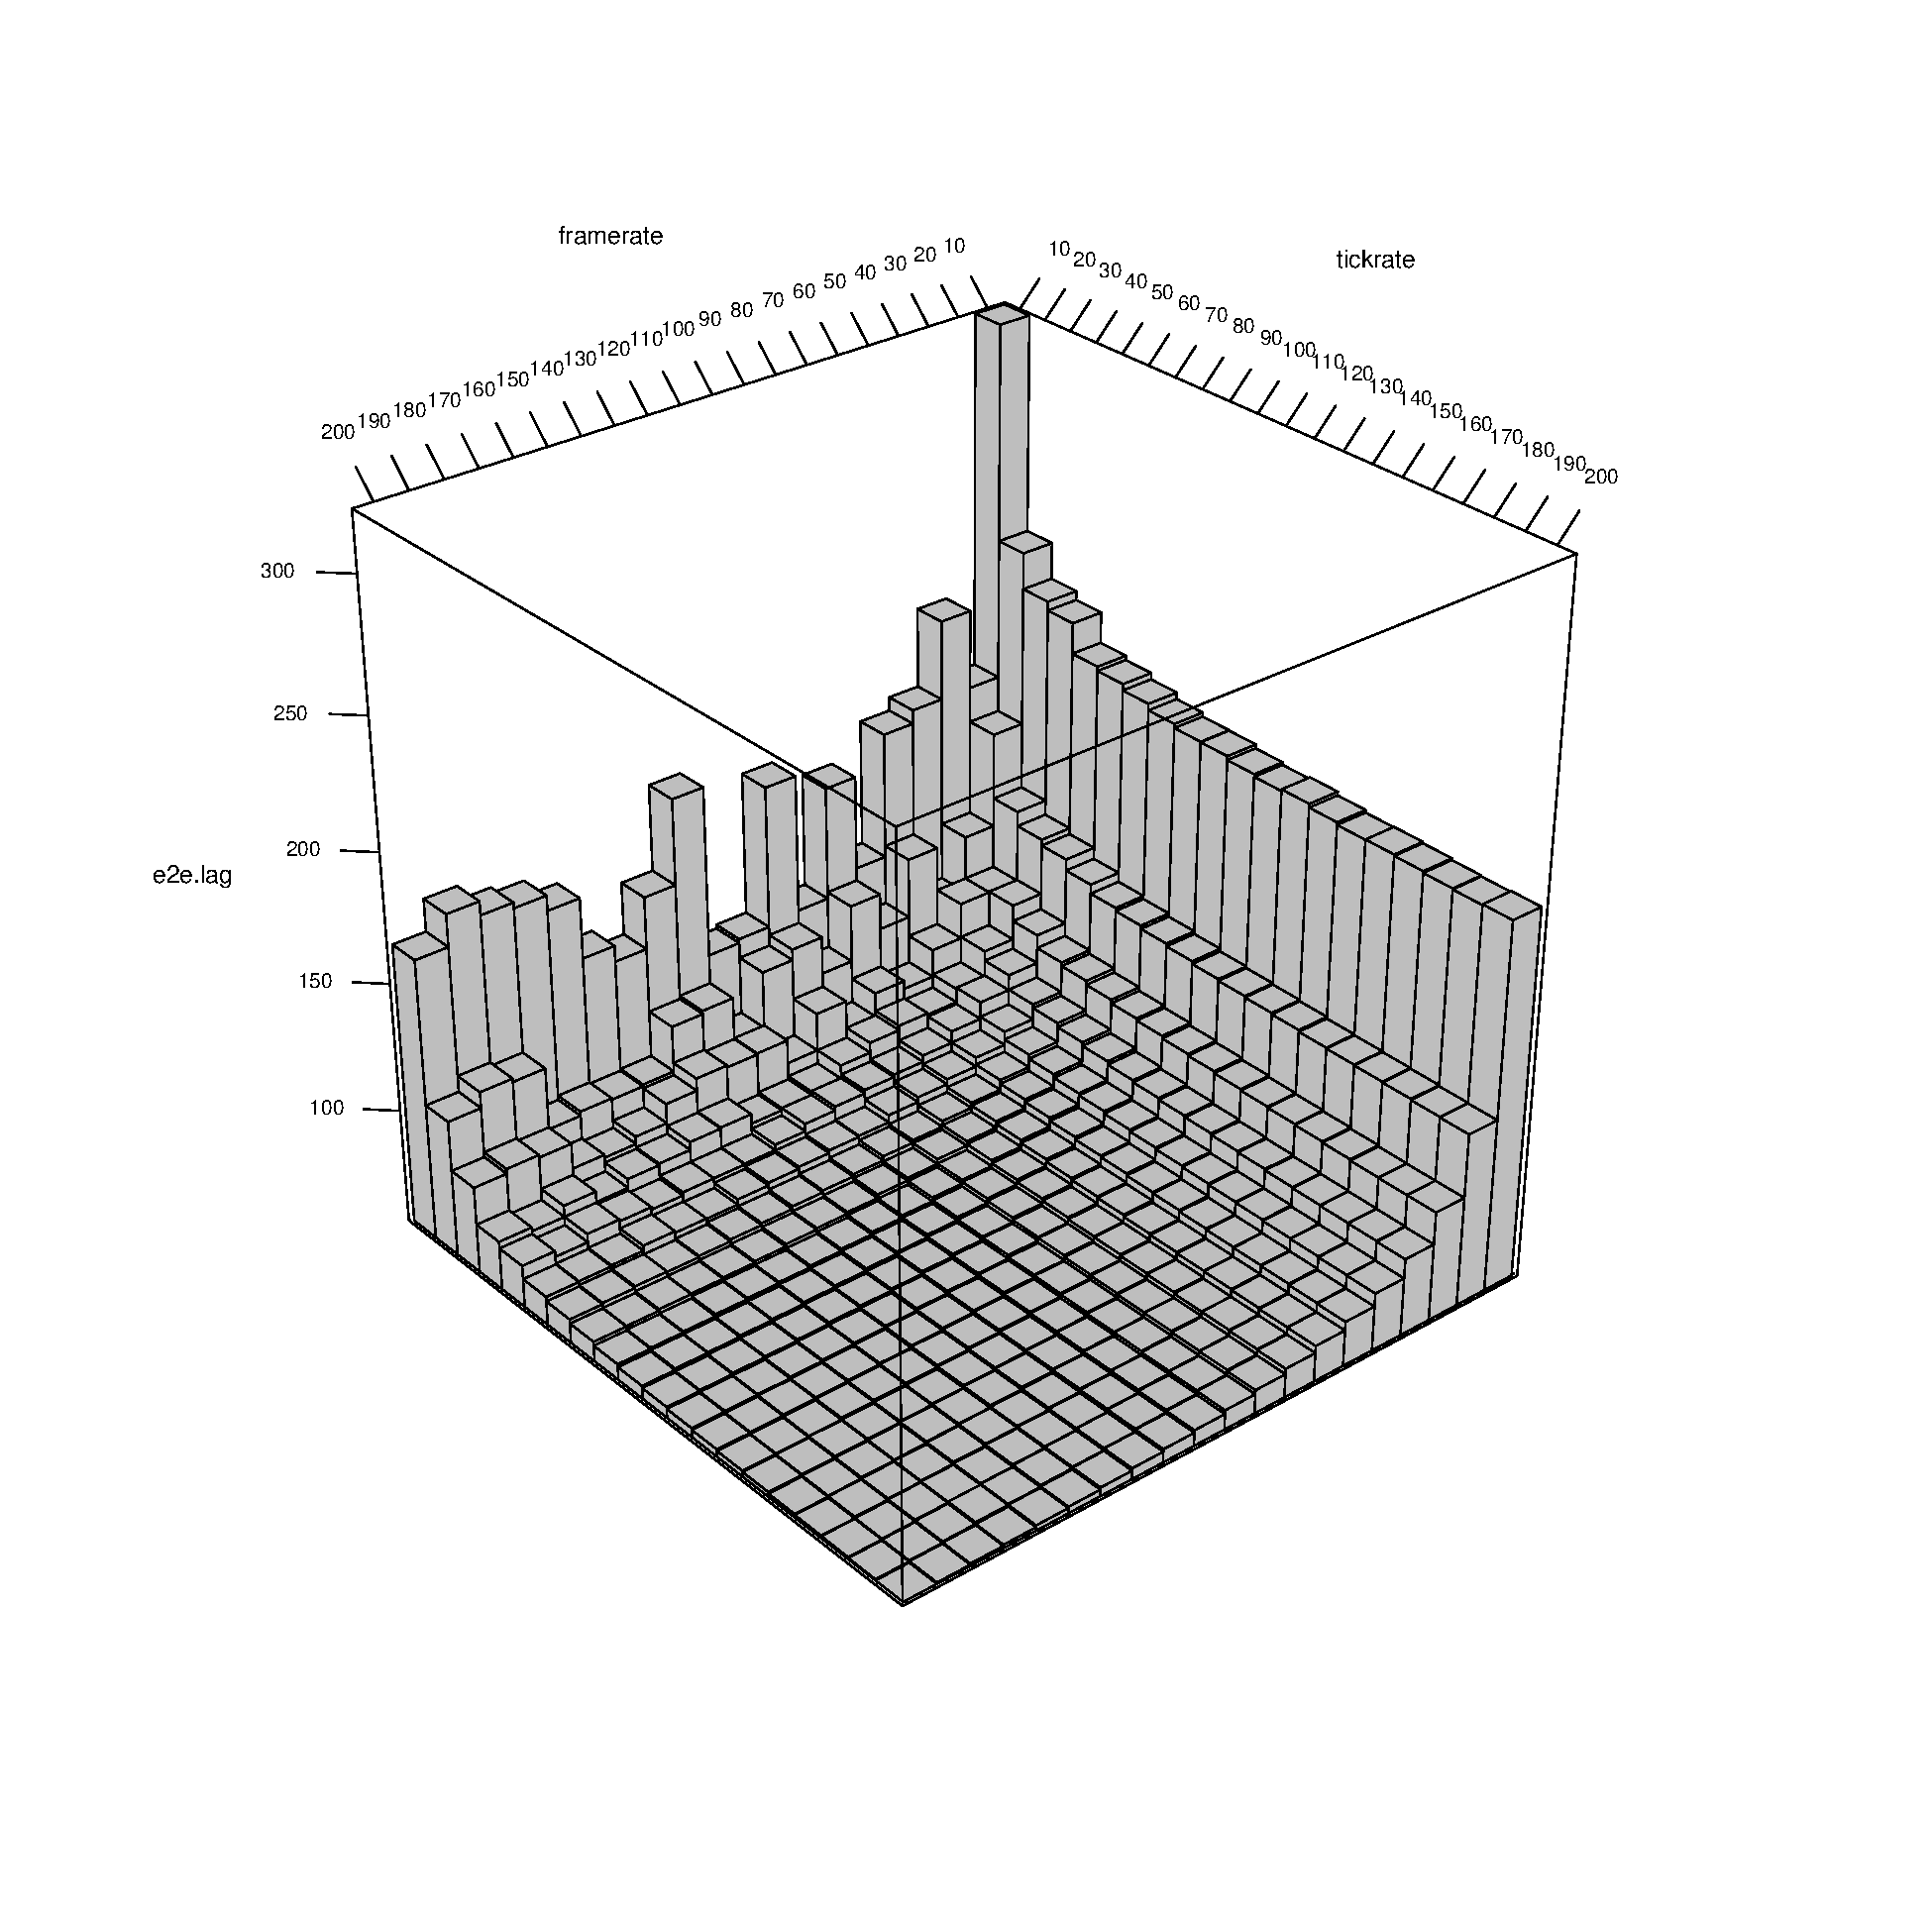
\includegraphics[width=1.0\columnwidth]{../simulation/visualization/e2e-lag-3dbars.pdf}
	\vspace{-15mm}
	\caption{3D bars representation of the influence of both the client's framerate and the server's tickrate on the end-to-end lag in the online game scenario.}
\label{fig:3dbars-framerate-tickrate-lag}
\end{figure}

Figure~\ref{fig:3dbars-framerate-tickrate-lag} shows a 3D bar plot of the influence of both the framerate and the tickrate on this scenario. Typical values for the framerate and tickrate are depicted here. Two things can be noted here. First, the framerate seems to have a larger influence on the lag than the tickrate. And second, the network delay is almost completely masked for low values of both framerate and tickrate, which dominate the resulting end-to-end lag. Only if both rates are high enough the network delay will play a more significant role.

This masking effect has large implications for video games and video game evaluations. Many of them exclusively examine the influence of just the network delay, without considering other influence sources to the end-to-end lag. This example demonstrates that this might not be the best course of action. It could also be assumed that this effect shifts to lower values of the frame- and tickrates when a higher network delay is examined.

A further property to note in this scenario is the much larger variance in the framerate dimension when compared to the tickrate. This can also have practical implications for video game studies. Experiments that examine the influence of the framerate need to have a very high repetition rate to keep the variance low and provide meaningful results.


%%%%%%%%%%%%%%%%%%%%%%%%%%%%%%%%%%%%%%%%%%%%%%%%%%%%%%%%%%%%%%%%%%%%%%%%%%%%%%%%
\subsection{Cloud Gaming}

Finally, the case of Cloud Gaming is also reconstructed as a simulation scenario for a hypothetical single-player game without any network interactions itself. To this end, the tickrate has been removed, but instead a constant encode (\SI{15}{\milli\second}) and decode delay (\SI{5}{\milli\second}) is in place at the game streaming server and client respectively. As the video frames are now rendered at the server, they need to be transported back to the client first. 
Without knowing the connection's throughput and absolute values for the frame sizes, the simulation simply applies an upper limit for the transmission duration, namely once again the frame's duration, or the inverse of the framerate. For the actual propagation delay, the same values as for the online game are used.

\begin{figure}[!t]
	\centering
	%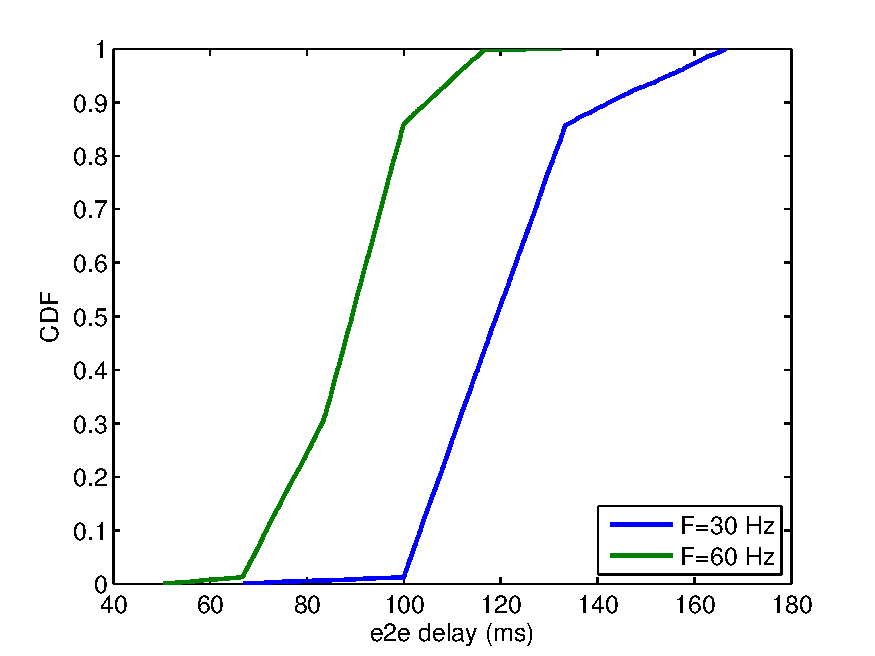
\includegraphics[width=1.0\columnwidth]{images/e2e-delay-sim.pdf}
	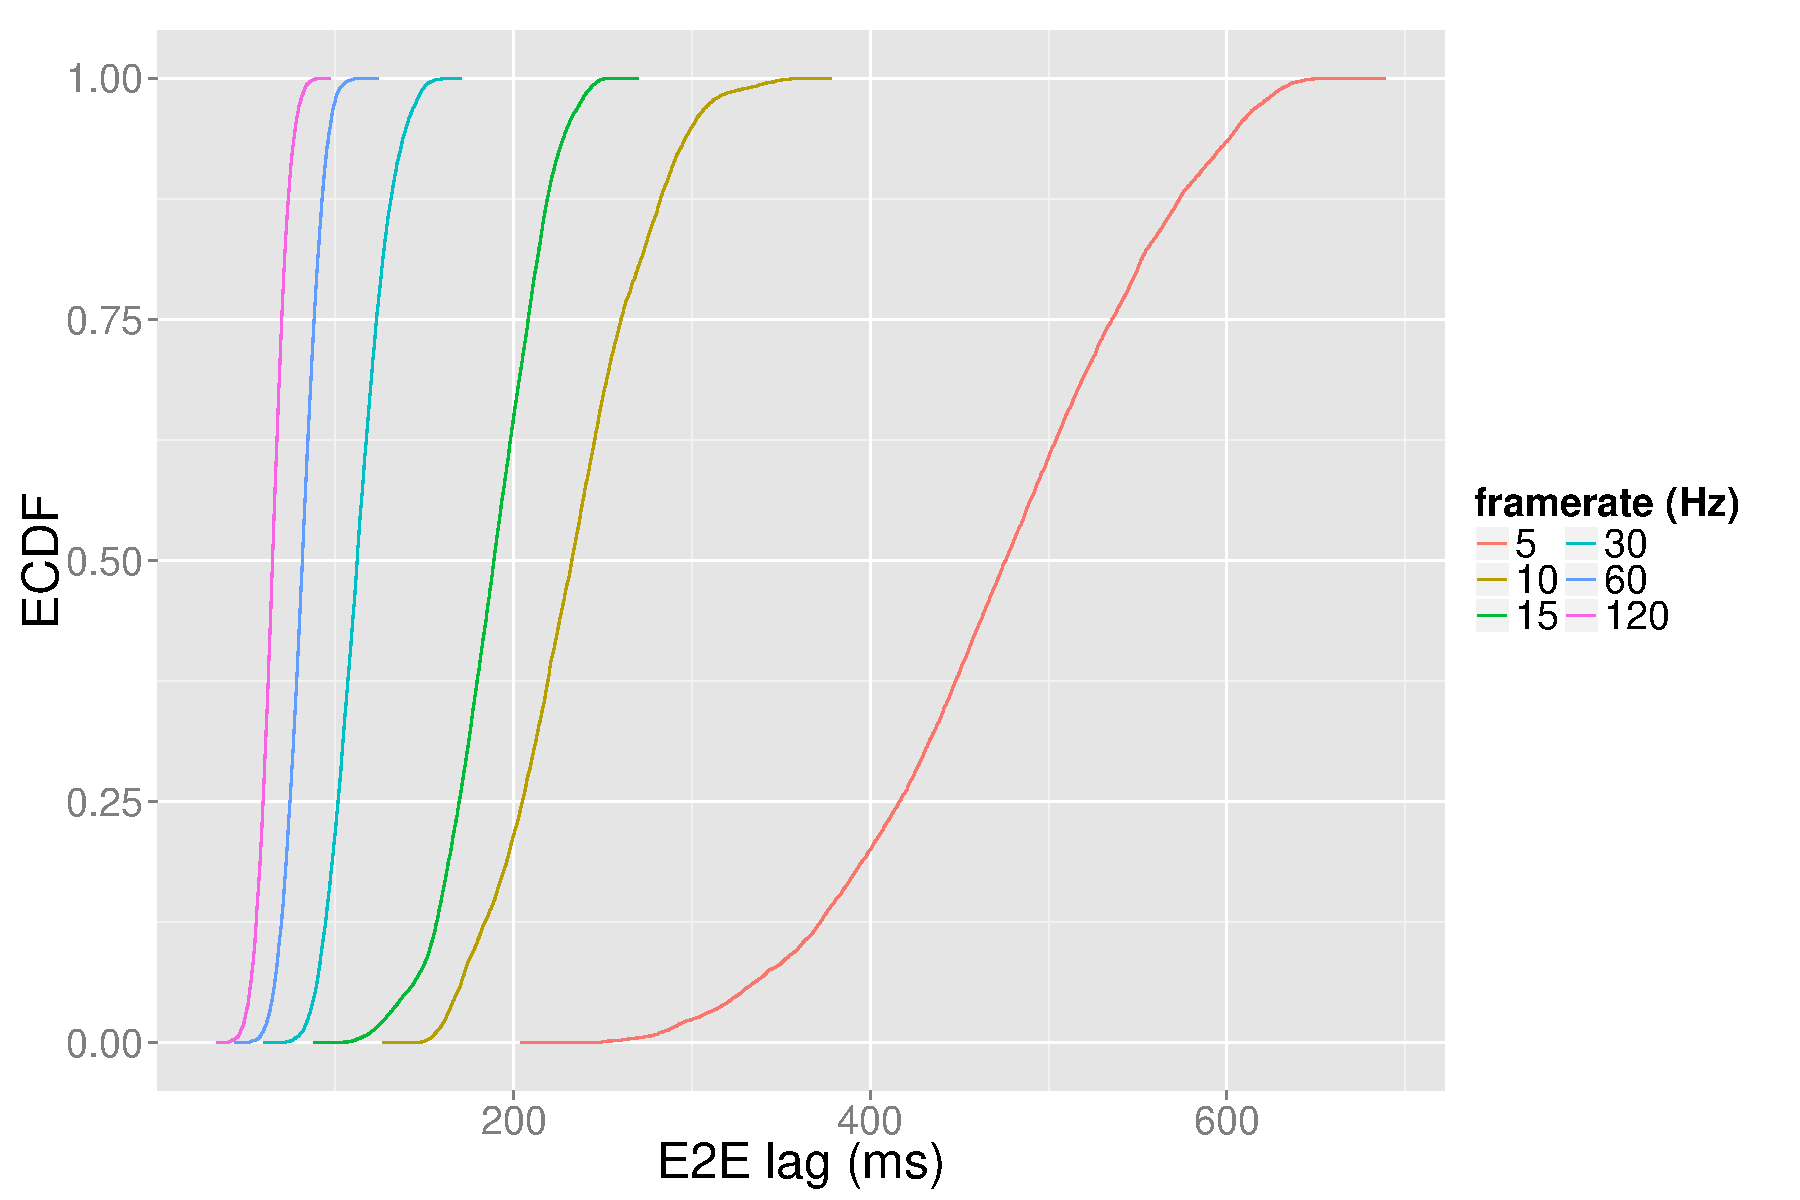
\includegraphics[width=1.0\columnwidth]{../simulation/visualization/cloudgaming-lag-cdf.pdf}
	\caption{\acrshort{ECDF} of the influence of the server's rendering and streaming framerate on the end-to-end lag in the cloud gaming scenario.}
\label{fig:cloud-e2e-delay-sim}
\end{figure}

In Figure~\ref{fig:cloud-e2e-delay-sim} the results of this Cloud Gaming scenario are shown as an \gls{ECDF} of the end-to-end lag for several framerates. Once again, the large influence of the framerate when compared to the network delay is evident. Past studies have relied on similarly low framerates when assessing the network influence on cloud gaming, which might be problematic, seeing the impact the framerate has on the end-to-end lag here. 
Similarly, these results can provide guidelines for implementors of cloud gaming to factor in the framerate in their calculations accordingly.


%%%%%%%%%%%%%%%%%%%%%%%%%%%%%%%%%%%%%%%%%%%%%%%%%%%%%%%%%%%%%%%%%%%%%%%%%%%%%%%%
\subsection{Discussion}

The three scenarios presented here serve to provide initial insights into the complex interactions of the end-to-end lag. Although the underlying abstract model adopts some simplifications and some properties are not factored in yet, the results are still very revealing.
Using the model and simulator as baseline, one can get a good estimation of the expected video game \gls{QoS} values. Alternatively, it can help in choosing representative games for select scenarios.

% Ultimately, to capture any and all latency sources in gaming you would need to rely on external recording gear.
% With modified input: zero latency and visible input detection (e.g. solder some LEDs to the buttons)

% Also Arduino with photodiode method described in \cite{beyermethod}
% Both this and camera method also work for closed game consoles


%%%%%%%%%%%%%%%%%%%%%%%%%%%%%%%%%%%%%%%%%%%%%%%%%%%%%%%%%%%%%%%%%%%%%%%%%%%%%%%%
%\subsection{Evaluated Metrics}

%%%%
%\subsubsection{Frame Rates and Frame Times (i.e. frame IAT)}
%i.e. frame IAT
%Reasoning for frame IAT and the negligence of past investigations
%%%%
%\subsubsection{Total and additional end-to-end latency}
%physical controller input to in-game reaction
%different in-game actions have already difference in latency, therefore need to test various actions for a complete picture
%Also discuss RTT as Hz (1/RTT) as measure for interactivity


%%%%%%%%%%%%%%%%%%%%%%%%%%%%%%%%%%%%%%%%%%%%%%%%%%%%%%%%%%%%%%%%%%%%%%%%%%%%%%%%
%\subsection{Reasonable Configuration/Setting Ranges to Test}

% Resolution: Minimum 720p, 1080p recommended, even higher is better (1440p or 2160p)
% Frame rate: 60 fps very much recommended, 30 absolute minimum,  120 or 144 can also be feasible
% Configure games to run at high or at least medium settings
% For console games: use the games intended settings for the console, never downscale the game or reduce the frame rate for streaming
% Assume no network latency higher than 200ms, preferably less than 100ms
% Assume typical access link conditions, i.e. no less than 10-16Mb/s



%Works only for general purpose computing devices with full access.
%Easiest method, but might not capture full end-to-end latency.
%FRAPS, OBS, DirectX Hooking, MSI Afterburner
%FCAT as hybrid solution with external capture card and computer


% \url{http://www.red.com/learn/red-101/high-frame-rate-video}


% articles:
% why frametimes
%     \url{https://techreport.com/review/21516/inside-the-second-a-new-look-at-game-benchmarking}

% Inside the second with Nvidia's frame capture tools
%     \url{https://techreport.com/review/24553/inside-the-second-with-nvidia-frame-capture-tools}

 % As the second turns: the web digests our game testing methods
 %    \url{https://techreport.com/blog/24133/as-the-second-turns-the-web-digests-our-game-testing-methods}

% GPU Reviews: Why Frame Time Analysis is important
%     \url{http://www.vortez.net/articles_pages/frame_time_analysis.html}

% Durante's Witcher 3 analysis: the alchemy of smoothness
%     \url{http://www.pcgamer.com//durantes-witcher-3-analysis-the-alchemy-of-smoothness/}


% Analysing Stutter – Mining More from Percentiles
%     \url{https://developer.nvidia.com/content/analysing-stutter-%E2%80%93-mining-more-percentiles-0}

% fraps vs fcat method
%     \url{http://www.extremetech.com/gaming/154089-after-almost-20-years-gpu-benchmarking-is-moving-past-frames-per-second}

% FRAPS + FRAFS
% \url{http://www.fraps.com/}
% \url{http://sourceforge.net/projects/frafsbenchview/}
% \url{http://www.5group.com/wordpress/2012/07/14/gpu-mist-pre-release-1-0-rc1/}

% issue: Fraps measures the flip queue input rather then the actual render output frames which is fine when measuring FPS but is rather poor if you want to measures actual frame times and analyze microstutter.


% NVIDIA FCAT
% \url{http://www.geforce.com/hardware/technology/fcat}
% \url{http://www.overclockers.com/nvidias-fcat-gpu-testing-pursuing/}


% Valve for Linux GL Games
% \url{https://github.com/ValveSoftware/voglperf}

% Info über MSI Afterburner overlay? oder GF experience? GPU-Z? Rivatuner Statistics Server?
% \url{http://www.overclock.net/a/how-to-use-rivatuner-afterburner-on-screen-display-and-more}



% \url{https://en.wikipedia.org/wiki/Game_classification}
% \url{https://en.wikipedia.org/wiki/Video_game_genre}
% \url{https://en.wikipedia.org/wiki/List_of_video_game_genres}

